\section{Background and Definitions}

\subsection{Software Security}
\eduard{introduce Software Security and then elaborate on the properties}
\newline
Jeff Hughes and George Cybenko~\cite{Hughes2013QuantitativeMA} identify three elements for computing system threats to existing:
\begin{itemize}
    \item inherent system susceptibility;
    \item the access of the threat to the susceptibility;
    \item the capability of threat to exploit the susceptibility.
\end{itemize}
Securing the system in the first place can reduce the susceptibility to the threat. The concept of security in computing systems encompasses three attributes: \textit{availability}, \textit{integrity}, and \textit{confidentiality}~\cite{concepts_secure_computing}. The \textit{IEEE Standard Glossary of Software Engineering Terminology}~\cite{standard_terms} defines the first two attributes as follows:

\theoremstyle{definition}
\begin{definition}[Availability]
\textit{``The degree to which a system or component is operational and accessible when required for use."}
\end{definition}

\theoremstyle{definition}
\begin{definition}[Integrity]
\textit{``The degree to which a system or component prevents unauthorized access to, or modification of, computer programs or data."}
\end{definition}

The National Institute of Standards and Technology (NIST) defines the last attribute as following~\cite{nist_glossary}:

\theoremstyle{definition}
\begin{definition}[Confidentiality]
\textit{``Preserving authorized restrictions on information access and disclosure, including means for protecting personal privacy and proprietary information."}
\end{definition}

Thus, accommodating a system with \ac{CIA} properties dictates its level of security. Jeff Hughes and George Cybenko~\cite{Hughes2013QuantitativeMA} claim that absolute CIA is unachievable as systems inevitably will have design trade-offs resulting in inherent weaknesses that can manifest, for instance, faults. In software, the concept of security is about designing fault-free and fault-tolerant software so it can continue functioning correctly even under attack~\cite{McGraw2004SoftwareS}. Software security also has an educational component requiring developers, architects, and users to follow best practices in software engineering and its usage. 

\subsection{Software Security Faults}
A \textit{fault} is the root cause of an \textit{error} that may lead to \textit{failure}(s)~\cite{taxonomy_security_flaws}. A fault can be internal or external to a system. The former concerns its internal state, while the latter is its external state, perceivable at the interface of a system. The \textit{IEEE Standard Glossary of Software Engineering Terminology}~\cite{standard_terms} includes the following definitions for the previous terms: 

\theoremstyle{definition}
\begin{definition}[Fault]
\textit{"An incorrect step, process, or data definition in a computer program."}. 
\end{definition}

\theoremstyle{definition}
\begin{definition}[Error]
\textit{"A human action that produces an incorrect result." (this definition is assigned to the word ``mistake'')}. 
\end{definition}

\theoremstyle{definition}
\begin{definition}[Failure]
\textit{"The inability of a system or component to perform its required functions within specified performance requirements")}. 
\end{definition}

%\begin{remark}
%The term bug is interchangeable with terms of fault and defect.
%\end{remark}

Figure~\ref{fig:fault_chain} depicts the manifestation mechanism of fault, error, and failure. It starts when a computation activates the fault, and the system enters an incorrect state. In that state, the error occurs as the system deviates from its intended functionality. An error propagates until it passes through the system-user interface, then becomes a \textit{failure}.

\begin{figure}[!h]
	\centering
    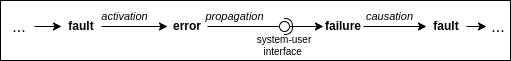
\includegraphics[width=0.95\textwidth]{figures/chapter_2/fault_pathology.drawio.png}
	\caption{The manifestation chain of a fault (\textit{cf.} \cite{concepts_secure_computing}).}
	\label{fig:fault_chain}
\end{figure}

%Catolino \textit{et al.}~\cite{Catolino2019NotAB} use the term bug to classify both development and operational faults in software. Moreover, the authors introduce a taxonomy of common root causes built from reports for software faults, including a class for software faults with security character. 

Faults cause expected scenarios not to run and turn into security faults when they compromise a system's security attributes, \textit{i.e.}, \ac{CIA}. The examples in Figure~\ref{fig:sec_fault_example} depicts the difference. The fault in listing~\ref{bug_ex} does not allow the \textit{pixels} variable to increment. On the other hand, the \textit{security fault} in listing~\ref{vuln_ex} results from wrong bounds-checking the \textit{for} cycle and subjects the system to a memory error. The error can be exploited by loading shell code into the allocated buffer memory, exposing the system to potential malicious use cases. A security fault that is accessible and exploitable is a \textit{vulnerability}. We will elaborate on vulnerabilities in section~\ref{sec:bg_vulns}.
\newline

% ############################## EXAMPLES ########################################
\begin{figure}[!htbp]
    \centering
    \noindent\begin{minipage}{0.48\textwidth}
        % ############################ BUG EXAMPLE ########################################
        \begin{lstlisting}[language = C, numbers = none, escapechar = !, linewidth=0.9\linewidth, basicstyle = \small, backgroundcolor=\color{lightgray}, frame=tb, caption={Fault example (\textit{cf.} \cite{Jason:2000}).}, captionpos=b, label=bug_ex, numbers=left, stepnumber=1]
for (i=0; i<numrows; i++)
    for (j=0; j<numcols; j++)!\textcolor{red}{;}!!\tikz[remember picture] \node [] (a) {};!
        pixels++;
        \end{lstlisting}
    \end{minipage}
    \begin{minipage}{0.45\textwidth}
        % ########################### VULN EXAMPLE ########################################
        \begin{lstlisting}[language = C++, numbers = none, escapechar = !, linewidth=\linewidth, basicstyle = \small, backgroundcolor=\color{lightgray}, frame=tb, caption={Security fault example (\textit{cf.} \cite{Castro:2016}).}, captionpos=b, label=vuln_ex, numbers=left, stepnumber=1] 
void vuln(){
 	int i;
 	int buf[128];
 	
 	for (i=0; !\textcolor{red}{i <= 128}!; i++) !\tikz[remember picture] \node [] (b){};!
 	    cin >> buf[i];
}
        \end{lstlisting}
    \end{minipage}
    \begin{tikzpicture}[remember picture, overlay,
        every edge/.append style = { ->, thick, >=stealth,
                                      darkgray, dashed, line width = 1pt },
        every node/.append style = { align = center, minimum height = 10pt,
                                     font = \bfseries, fill= red!20},
                      text width = 2.5cm ]
      \node [above left = 0.9cm and -0.5cm of a, text width = 2.cm]  (A) {accidental semicolon};
      \node [above left = 1.1cm and 0.5cm of b,text width = 2.cm] (B) {off-by-one error};
      \draw (A.south) + (0.55, 0) coordinate(x1) edge (x1|-a.north);
      \draw (B.south) + (0, 0) coordinate(x1) edge (x1|-b.north);
    \end{tikzpicture}
    \caption{Example of a fault (left) and a security fault (right).}
    \label{fig:sec_fault_example}
\end{figure}

To enforce security policies, Landwehr \textit{et al.}~\cite{taxonomy_security_flaws} characterize security faults by three dimensions: \textit{genesis}, \textit{time of introduction}, and \textit{location}. The former answers how a security fault entered the system and whether it can be \textit{intentional} or \textit{inadvertently}. The time of introduction of a security fault aligns with the \ac{SDLC}. It is determined by one of the three different phases in the life cycle of a system: \textit{development}, \textit{maintenance}, or \textit{operational}. For Avizienis \textit{et al.}~\cite{concepts_secure_computing}, the time of introduction resumes with the \textit{development} and \textit{operational} phases, as the latter covers maintenance. During development, all activities up to the release of the initial version of the system can originate security faults, for instance, by including additional mechanisms to the specification for testing the system. During the maintenance phase, activities leading to security faults are often attributable to malicious intrusion or incompetence of the programmer in understanding the system. During the operational phase, unauthorized or unsafe modifications to the system can introduce security faults — \textit{e.g.}, installing virus programs. Finally, a security fault starts manifesting in a location in the system, which can be in the \textit{software} or \textit{hardware}.

Our focus regarding genesis is on accidental security faults as in the latter, the detection approaches are much less likely to help, and measures concern the trustworthiness of the programmers. Regarding the time of introduction and location, our concern is software security faults introduced during the development phase. These can originate in \textit{requirements and specifications}, \textit{source code}, or \textit{object code}. Software requirements and specifications only describe the design of a particular system and its functionality, source code is the actual implementation, and object code only represents the machine-readable form of the previous. We consider source code as we focus on avoiding faults in the software during its implementation to handle threats proactively.

A security fault in software can occur in one of the following software layers: \textit{operating system programs}, \textit{support software}, or \textit{application software}. Similarly, Khwaja \textit{et al.}~\cite{Khwaja2020ASF} identify, based on mitigation techniques, the reach of security faults in software but only at two levels: \textit{operating systems} and \textit{software applications}. Security faults in the former can compromise system functions, such as process and memory management, and cause the most significant injury. Support and application software are programs outside the \ac{OS} boundary — \textit{e.g.}, editors and libraries. Support software has granted privileges, and a security fault in them can allow privilege escalation to gain further unauthorized access to the system. Application software has no special system privileges, but a security fault in them can still cause considerable damage within the storage of the victim. 

\subsection{Classes of Software Security Faults}
\eduard{TODO}